\section*{GUI}

Środowisko graficzne powstało w celu zobrazowania jak działa model w rzeczywistości. Zostało stworzone w języku Python z wykorzystaniem biblioteki PyGame. Działanie opiera się na zamianie obiektu board z biblioteki chess na plansze szachową z figurami, gdzie każda z nich jest w postaci zdjęcia z usuniętym tłem. Umożliwia również wykonywanie ruchów białymi figurami przez użytkownika. Interfejs graficzny dopuszcza i pokazuje tylko poprawne ruchy. W momencie gdy jest tura przeciwnika, wywoływany jest listener zwracający obiekt move. Taka struktura pozawala na bardzo łatwą implementację dowolnego algorytmu.

\begin{figure}[h]
\centering
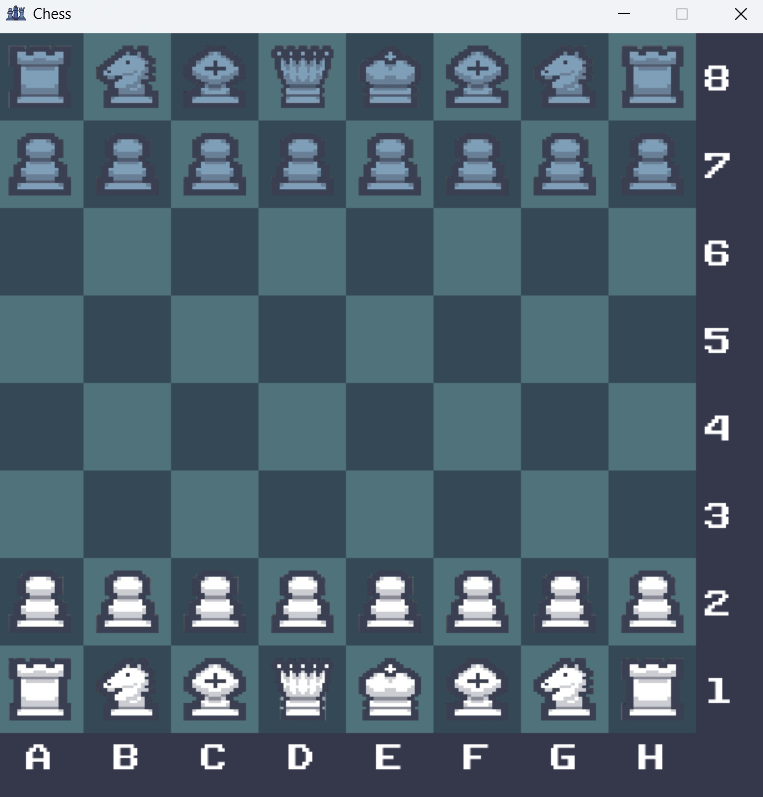
\includegraphics[width=0.4\textwidth]{images/gui_czyste.png}
\hspace{1cm}
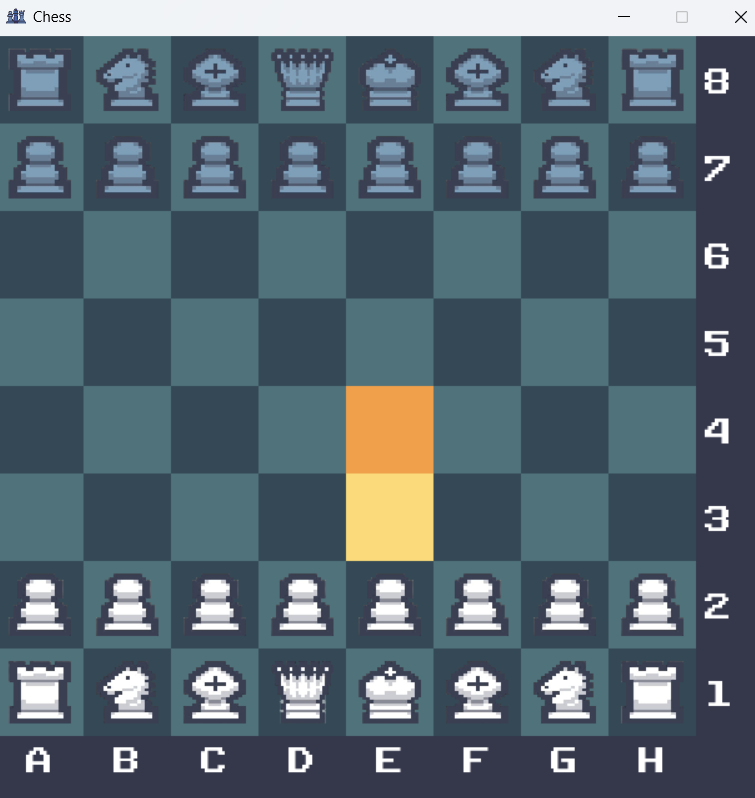
\includegraphics[width=0.4\textwidth]{images/gui_ruch.png}
\caption{intefejs graficzny}
\end{figure}

\lstset{style=codeListingStyle}
\begin{lstlisting}[
    language=Python, 
    caption=Przykładowe użycie gui,
    inputencoding=utf8
]
# obiekt board na ktorym dziala cala gra
board = BoardPlus() 

@torch.no_grad()
def algorithm():
    prob = chess_mctsnn.AMCTS(200, net).search(board)
    move_id = np.argmax(prob)
    move_mcts = board.decode_move(move_id)
    # zmiana perspektywy ruchu na czarne
    move_mcts = board.change_move_perspective(move_mcts)
    return move_mcts

game = chessGUI(board)
game.add_computer_algorithm_listener(algorithm)
game.run()
\end{lstlisting}